\label{section:introduction}
%%%%%%%%%%%%%%%%%%%%%%%%%%%%%%
This manual provides a short description of the \fitter\ program 
which can be used to determine unpolarised parton density functions 
(PDFs) using deep inelastic scattering (DIS) data and other processes such as 
Drell-Yan, jet or ttbar processes.
The parton density functions are needed to calculate cross sections
for the $ep$ and $pp$ colliders and thus required for interpetation
of the data collected at the LHC.
% The \fitter\ program were used to determine the HERA1.0 PDF set~\cite{h1zeus:2009wt}.

A schematic structure of the \fitter\ is illustrated in Fig.~\ref{fig:flow}
\begin{figure}
\begin{center}
\caption{Schematic Structure of the \fitter\ program}
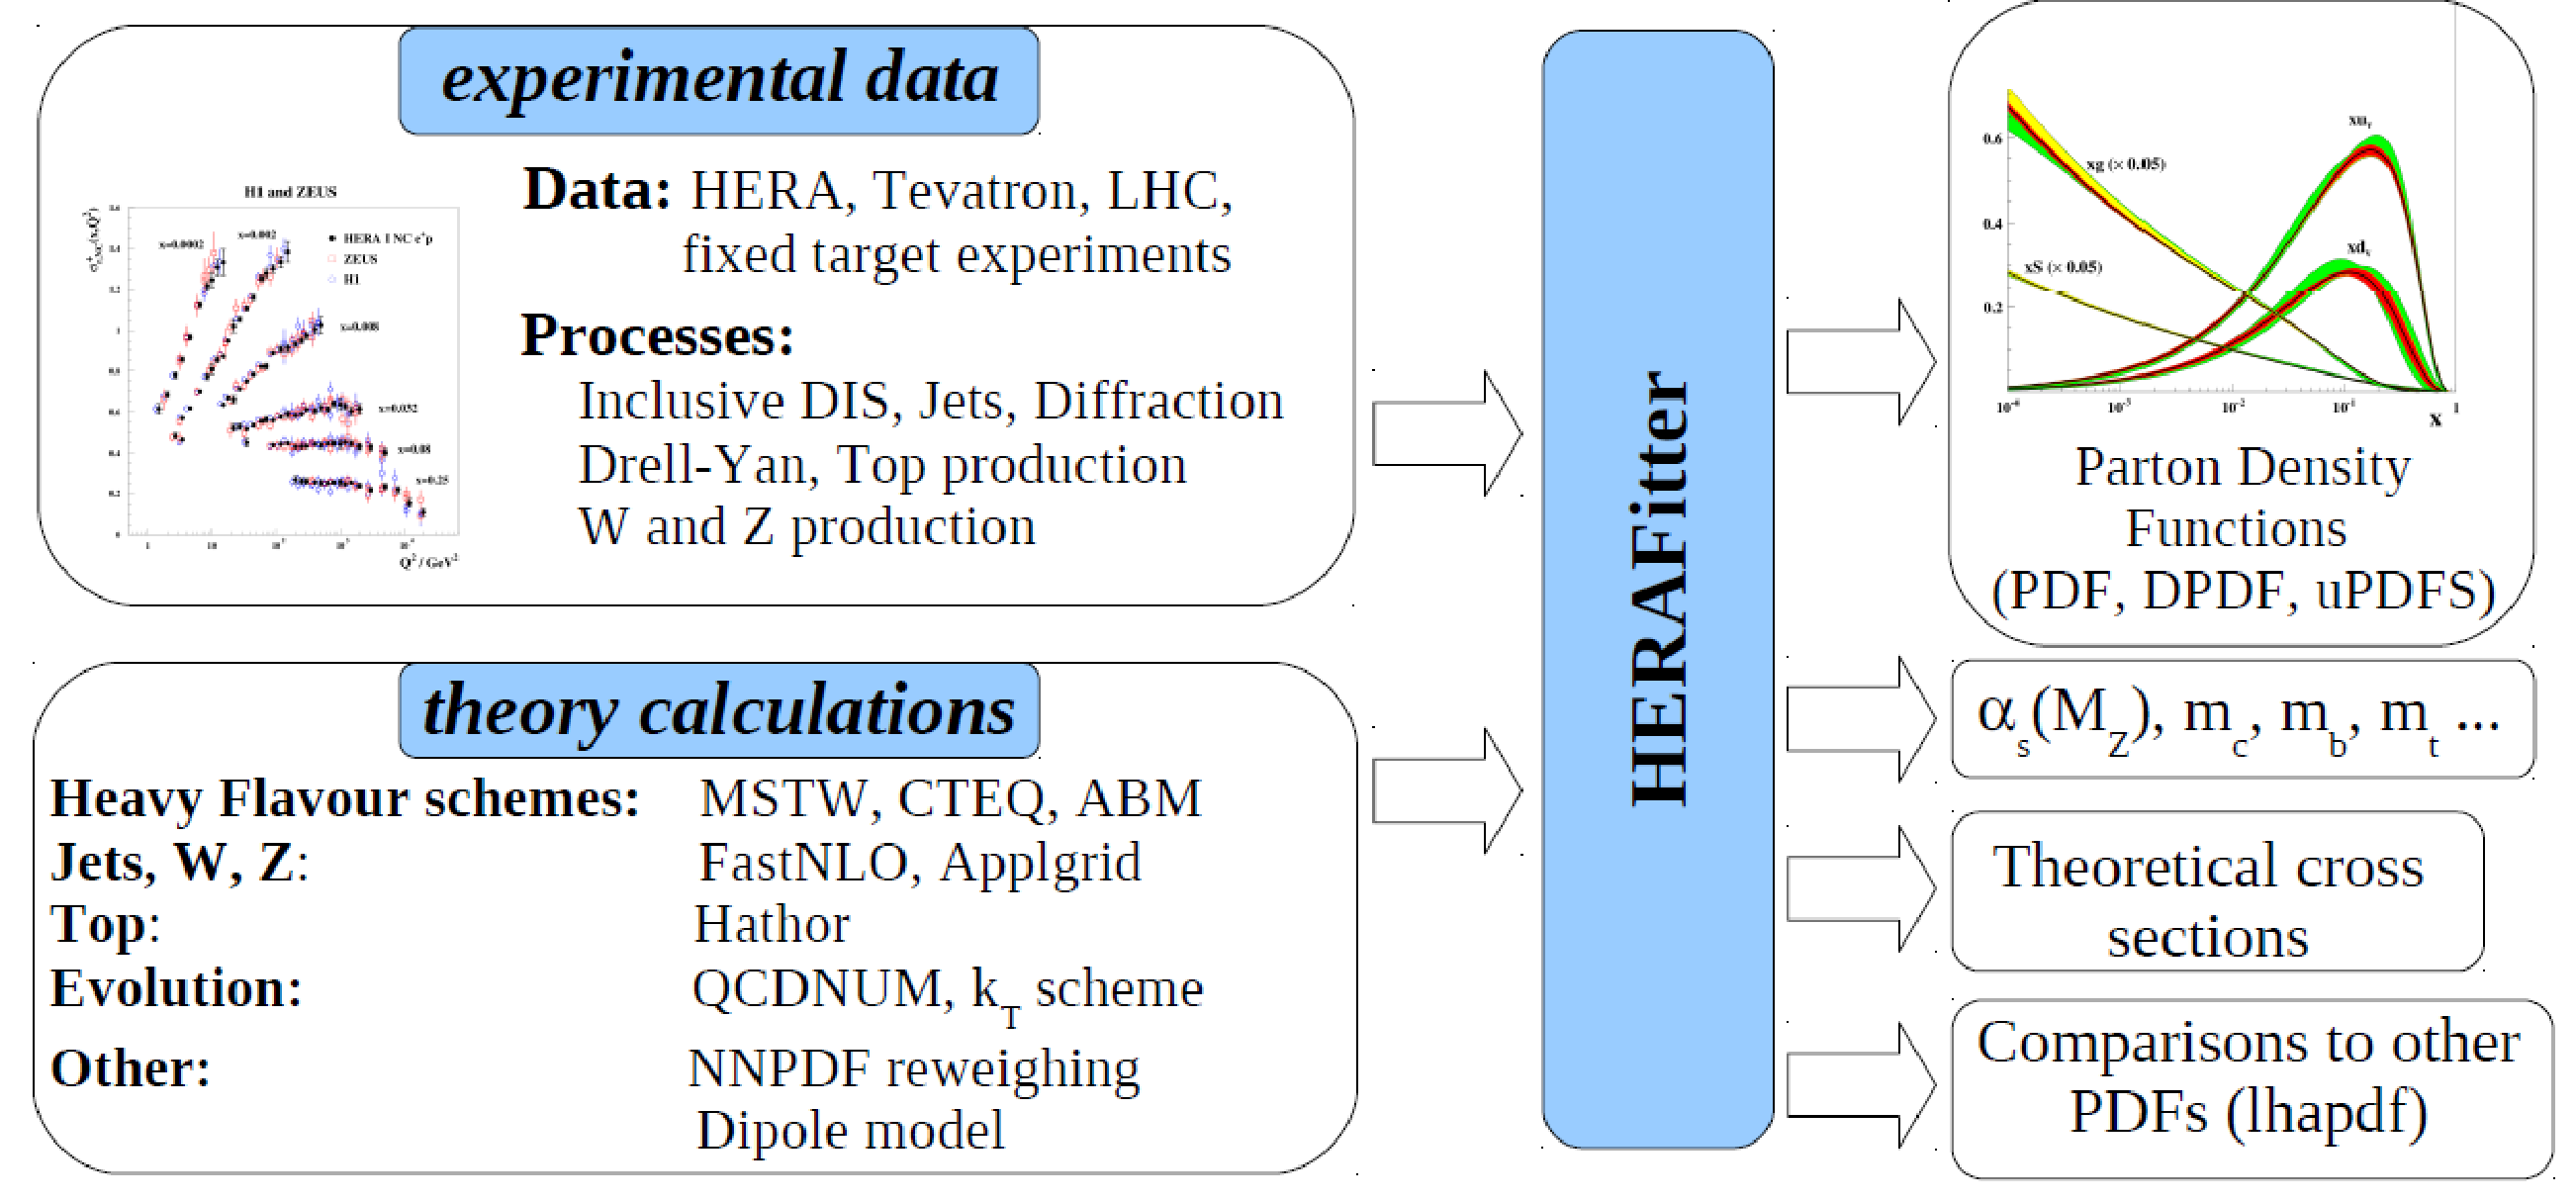
\includegraphics[width=0.75\linewidth]{figures/flow.pdf}
\end{center}
\label{fig:flow}
\end{figure}

The manual is structured such that it first dedcribes briefly the theoretical input and fit choices
and then it provides the user manual with concrete examples.
Therefore, the manual begins with program installation instructions for different scenarios (section~\ref{sec:install}), followed by a brief discussion of the theoretical calculation
used in the program (section~\ref{sec:theory}) continued by a description of the
PDF parameterisation (section~\ref{sec:pdfparam}) and various $\chi^2$ functions used in the
minimisation (section~\ref{sec:chi2}). A description of the program steering cards and
the output options is given in section~\ref{sec:man}.

